\documentclass[11pt,a4paper]{article}
\usepackage{ifpdf}
\usepackage[utf8]{inputenc}
\usepackage[francais]{babel}
\usepackage[T1]{fontenc}
\usepackage[nottoc, notlof, notlot]{tocbibind}
\usepackage[unicode=true,pdftex,colorlinks=true,linkcolor=black,urlcolor=black,citecolor=black]{hyperref}
\usepackage{natbib}
\usepackage{graphicx}

\parindent 0.8cm
%\setlength{\parskip}{0.5em plus 0.2em minus 0.2em}

\title{Projet Androïd : Rapport}
\author{Anthony \textsc{Caillaud} Manoël \textsc{Fortun} Vincent
\textsc{Pottier} Charles \textsc{Dejean}}
\date{\today}
\ifpdf
\pdfinfo {
/Author (Anthony Caillaud Manoël Fortun Vincent Pottier Charles Dejean)
/Title (RoadMapJDR)
/Subject (RoadMapJDR)
/Keywords ()
/CreationDate (D:20100329212218)
}
\fi


\begin{document}

\maketitle

\clearpage
\tableofcontents
\clearpage
\section{Introdution}

Ce rapport reprend la suite de la Roadmap que nous avions définis pour notre
projet d'ihm autour d'une application pour le jeu de rôle sous androïd.
Dans la continuité du précédent rapport nous avons suivis la méthode LUCID pour
la conception et réalisation de notre application. Ce rapport reprendra donc là
ou nous nous étions arrêté, c'est à dire à l'étape 2 de LUCID, et finira à 6
avec le plan d'évaluation si nous étions dans un contexte réel.
Avant chaque étape nous rappelerons les enjeux de l'épate et notre
interprétation.

\clearpage

\section{Lucid 2}

\subsection{Définition}

Cette étape de la méthode permet de compléter la première étape, et donc de
receuillir en fonction des catégories d'utilisateur et du concept de
l'application les attentes des utilisateurs. D'obtenir aussi les choses qu'ils
jugent indispensable, la façon qu'ils auraient d'appréhender l'application via
des scénario, et donc les implications en termes de fonctionnalités.

\subsection{Approche des utilisateurs}

Nous avons soumis notre projet à des rolistes, des rolistes pas tous experts en informatique, 
le cliché des geeks informaticiens rolistes est loin d'être une vérité. Nous n'avons pas eut besoin 
vraiment de partionner les résultats et de les analyser séparément en fonction des catégories d'utilisateurs.\\

De plus nous avons pensé qu'interroger des gens totalement ignorant du jeu de rôle, mais connaissant
l'informatique ou les applications mobiles n'était pas pertinent. En effet séduire des gens "expert" en mobile
au jeu de rôle n'est pas le but de l'application et même si c'était son but ce n'est pas ainsi que l'on séduit des clients.
Donc cette partie de l'étude n'a pas été mené, c'est peut être un biais que nous n'aurions pas du prendre, mais 
l'intérêt nous semblait très limité.\\

Dans notre approche de l'étude des commentaires de futurs utilisateurs, nous avons pu nous rendre compte
au départ nos explications n'étaient pas toujours clair. En effet certain premier "client" nous ont demandé si
nous n'étions pas en train de faire un jeu. Par la suite nous avons mieux construit nos explications.\\

Dans les réponses que nous avons pu récolter il y a trois grand type de réaction commune, des réactions 
assez prévisible dans l'ensemble.\\

En général les gens trouvent que Joël il est tout petit.\\

La première réaction est celle des irréductibles, accrochés à la symbolique du support physique de leur dés et de
leurs fiches. Parce que lancer un téléphone sur un joueur c'est vachement plus onéreux que lui lancer ses dés. 
Même remarque sur le fait de poignarder un joueur avec téléphone plutot que le sacro saint crayon de bois servant à
l'édition de sa fiche.\\

Ensuite il y a les gens très enthousiaste par l'idée, du coté joueur et MJ qui sont intéressés
et souhaitent voir des choses comme la synchronisation facile avec ordinateur, 
des thèmes personnalisables en fonction du jeu. Des dés "physiques" et visuel, personnalisable aussi.\\

Classiquement il y a aussi les gens curieux de voir ce que ça va donner.\\

Passer ces premières réactions il y a quelques demandent particulières ou questions qui se sont posés.
Comme le fait de pouvoir convertir ses fiches en fiches papiers qui s'imprimeraient rempli comme des fiches
classique. La partie connectivité qui à été compliqué à expliquer, tant elle se rapproche d'un système de chat 
classique mais en étant éloigné, ce qui se ressent c'est le sentiment d'espionnage par le MJ.\\

Au niveau IHM pur, et concept lié, les gens ont tendance à penser que le support téléphone tout en
étant pratique est moins adapté qu'un tablette PC. Convaincre avec cette application peut être compliqué.
Nous avons pu nous rendre compte par cette étude mené autour de partie et dans la façon qu'on les joueurs 
d'utiliser leur fiche que la navigation entre différent niveau d'une fiche doit être rapide et simple. 
De même les éditions de certain composant de personnage comme son niveau de vie doivent être
très très rapide tant celà arrive souvent au cours d'une partie.\\

Celà nous à permis de compléter les UserStories que nous avions déjà commencé à définir.\\

\subsection{User Stories}

Cette partie regroupe donc nos scénarios construit en partie en amon de la phase de communication, et complété après
analyse des réactions clients.

\chapter{User Stories pour le composant dé}

En tant que Joueur, avec le composant de dés, je dois pouvoir lancer un nombre
de dé choisi et du type que je souhaite et je dois pouvoir voir le résultat
correct.
~

En tant que Joueur, avec le composant de dés, je dois pouvoir, après un jet de
dés, relancer les dés avec les mêmes caractéristiques.
~

En tant que Joueur, avec le composant de dés, je dois pouvoir changer le type de
dés ou le nombre

\clearpage


\subsubsection{User Stories pour la connectivité}

En tant que Joueur, avec le module Connectivité, je dois pouvoir rejoindre une
salle de chat.\\

En tant que Joueur, avec le module Connectivité, je dois pouvoir créer un salon
et devenir maître de salon.\\

En tant que Joueur, avec le module Connectivité, je dois pouvoir parler de façon
discrète (privée) à un autre joueur présent.\\

En tant que Joueur, avec le module Connectivité, je dois pouvoir choisir que
toutes mes conversations soient visibles par le maître de salon.\\

En tant que Joueur, avec le module Connectivité, je dois pouvoir choisir que
tous mes jets soient envoyés au Maître du salon.\\


En tant que Maître du salon, avec le module Connectivité, je dois pouvoir
choisir de ne pas voir les conversations ou les dés.\\

En tant que Joueur, avec le module Connectivité, je dois pouvoir ne pas être que
sur un salon.\\

En tant que Joueur, avec le module Connectivité, je dois pouvoir accéder à la
liste des gens sur le salon.\\

En tant que Joueur, avec le module Connectivité, je dois pouvoir, depuis ma
fiche, accéder rapidement au salon ou je suis connecté.\\



\subsubsection{User Stories pour le Joueur}

En tant que Joueur, dans la partie consultation de fiche, je dois pouvoir voir
les caractéristiques du personnage.\\

En tant que Joueur, dans la partie consultation de fiche, je dois pouvoir voir
les compétences du personnage.\\

En tant que Joueur, dans la partie consultation de fiche, je dois pouvoir voir
les autres informations du personnage, en fonction du jeu.\\

En tant que Joueur, dans la partie consultation de fiche, je dois pouvoir voir
les caractéristiques secondaires du personnage.\\

En tant que Joueur, dans la partie consultation de fiche, je dois pouvoir
sélectionner une caractéristique afin de pouvoir la modifier.\\

En tant que Joueur, dans la partie consultation de fiche, je dois pouvoir
sélectionner une compétence afin de pouvoir la modifier.\\

En tant que Joueur, dans la partie consultation de fiche, je dois pouvoir
sélectionner une caractéristique secondaire afin de pouvoir la modifier.\\

En tant que Joueur, dans la partie consultation de fiche, je dois pouvoir
passer d'une catégorie à une autre facilement.\\

En tant que Joueur, dans la partie consultation de fiche, je dois pouvoir
sélectionner la fiche consultée pour une autre partie.\\


\chapter{User Stories pour le MJ}

En tant que MJ, dans la partie fiche de joueurs, je dois pouvoir voir les
caractéristiques d'une feuille de joueur.
~

En tant que MJ, dans la partie fiche de joueurs, je dois pouvoir voir les
compétences d'une feuille de joueur.
~

En tant que MJ, dans la partie fiche de joueurs, je dois pouvoir voir les
caractéristiques secondaires d'une feuille de joueur.
~

En tant que MJ, dans la partie fiche de joueurs, je dois pouvoir voir les
pouvoirs d'une feuille de joueur.
~

En tant que MJ, dans la partie fiche de joueurs, je dois pouvoir voir les
barre de vie d'une feuille de joueur.
~

En tant que MJ, dans la partie fiche de joueurs, je dois pouvoir choisir une
feuille de joueur.
~

En tant que MJ, dans la partie fiche de pnjs, je dois pouvoir choisir une
feuille de pnj. ~

En tant que MJ, dans la partie fiche de pnj, je dois pouvoir voir les
caractéristiques d'une feuille de pnj.
~

En tant que MJ, dans la partie fiche de pnj, je dois pouvoir voir les
compétences d'une feuille de pnj.
~

En tant que MJ, dans la partie fiche de pnj, je dois pouvoir voir les
caractéristiques secondaires d'une feuille de pnj.
~

En tant que MJ, dans la partie fiche de pnj, je dois pouvoir voir les
pouvoirs d'une feuille de pnj.
~

En tant que MJ, dans la partie fiche de pnj, je dois pouvoir voir les
barre de vie d'une feuille de pnj.
~

En tant que MJ, dans la partie jet de dé, je dois pouvoir faire un jet à partir
d'une feuille de joueur.
~

En tant que MJ, dans la partie jet de dé, je dois pouvoir faire un jet à partir
d'une feuille de pnj.
~

En tant que MJ, dans la partie jet de dé, je dois pouvoir faire un jet de dé
quelconque, dans le système de l'univers.
~

En tant que MJ, dans la partie jet de dé, je dois pouvoir faire un jet de dé
quelconque, hors système.
~



\clearpage


\section{Lucid 3}

\subsection{Définition}

Cette étape de la méthode est la première étape visuelle, c'est à se moment là
que on se sert des infos compilées des précédentes étapes pour pouvoir dessiner
quelques chose qui aura un chance de plaire aux utilisateurs finaux.
On se sert des indications utilisateurs visuel, de ce qui est possible et des
users stories pour construire les interractions entre écran, enchainement.
Pendant cette étape il est très important que sur les exquisses d'interfaces il
n'y ait pas d'ambiguité possible, tout élément doit être nommé pertinement et
correspondre à quelque chose qui à du sens. Le label "accès fiche'' est
préférable au label "ponay''. 


\subsubsection{Esquisses interface}

Suite aux analyse nous avons fais des esquisses d'interface,
nous avons travaillé grâce aux outils googledocs et en particulier l'outil drawning.
Ces interfaces de l'application et l'enchainement des écrans ont été définis à l'aide 
de l'analyse des besoins utilisateurs et de leur façon d'utiliser une fiche, ainsi que l'intégration de
toutes nos fonctions.\\

Pour l'interface nous choisis très simplement dans un premier temps de 
s'attarder uniquement sur l'aspect fonctionnel. L'aspect fonctionnel niveau ergonomie 
était un réel travail compte tenu du nombre d'information à afficher et à rendre éditable, utilisable facilement.\\

En ce qui concerne le look and feel, il y a un fort souhait utilisateur de personnsalisation de celle-ci, 
mais au départ le look and feel sera celui existant de base sous android. Le look and feel pouvant impacter
la taille des éléments à afficher, ça sera une étape gérer dans une prochaine version de notre application.\\

\begin{figure}[h]
  	
  		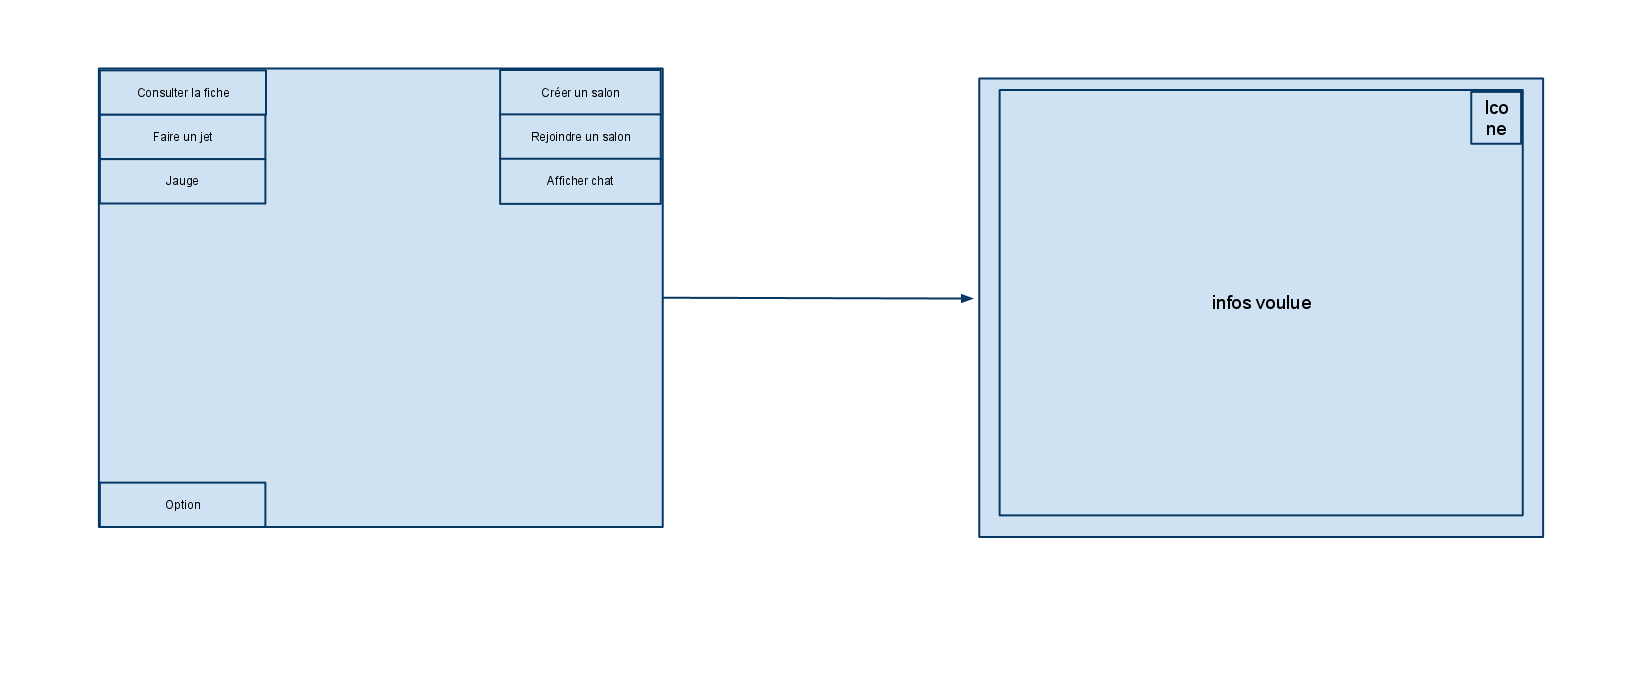
\includegraphics[height=14cm,width=15cm]{image/screen1.png}
  		\caption{Ecran démarage/concept}
  		\label{screen1}
\end{figure}

Sur la capture \ref{screen1} on peut voir le concept général, avec le transfert sur un écran suivant
son choix, pas de chose qui s'affiche en sur impression des premiers écrans.

\begin{figure}[h]
  	
  		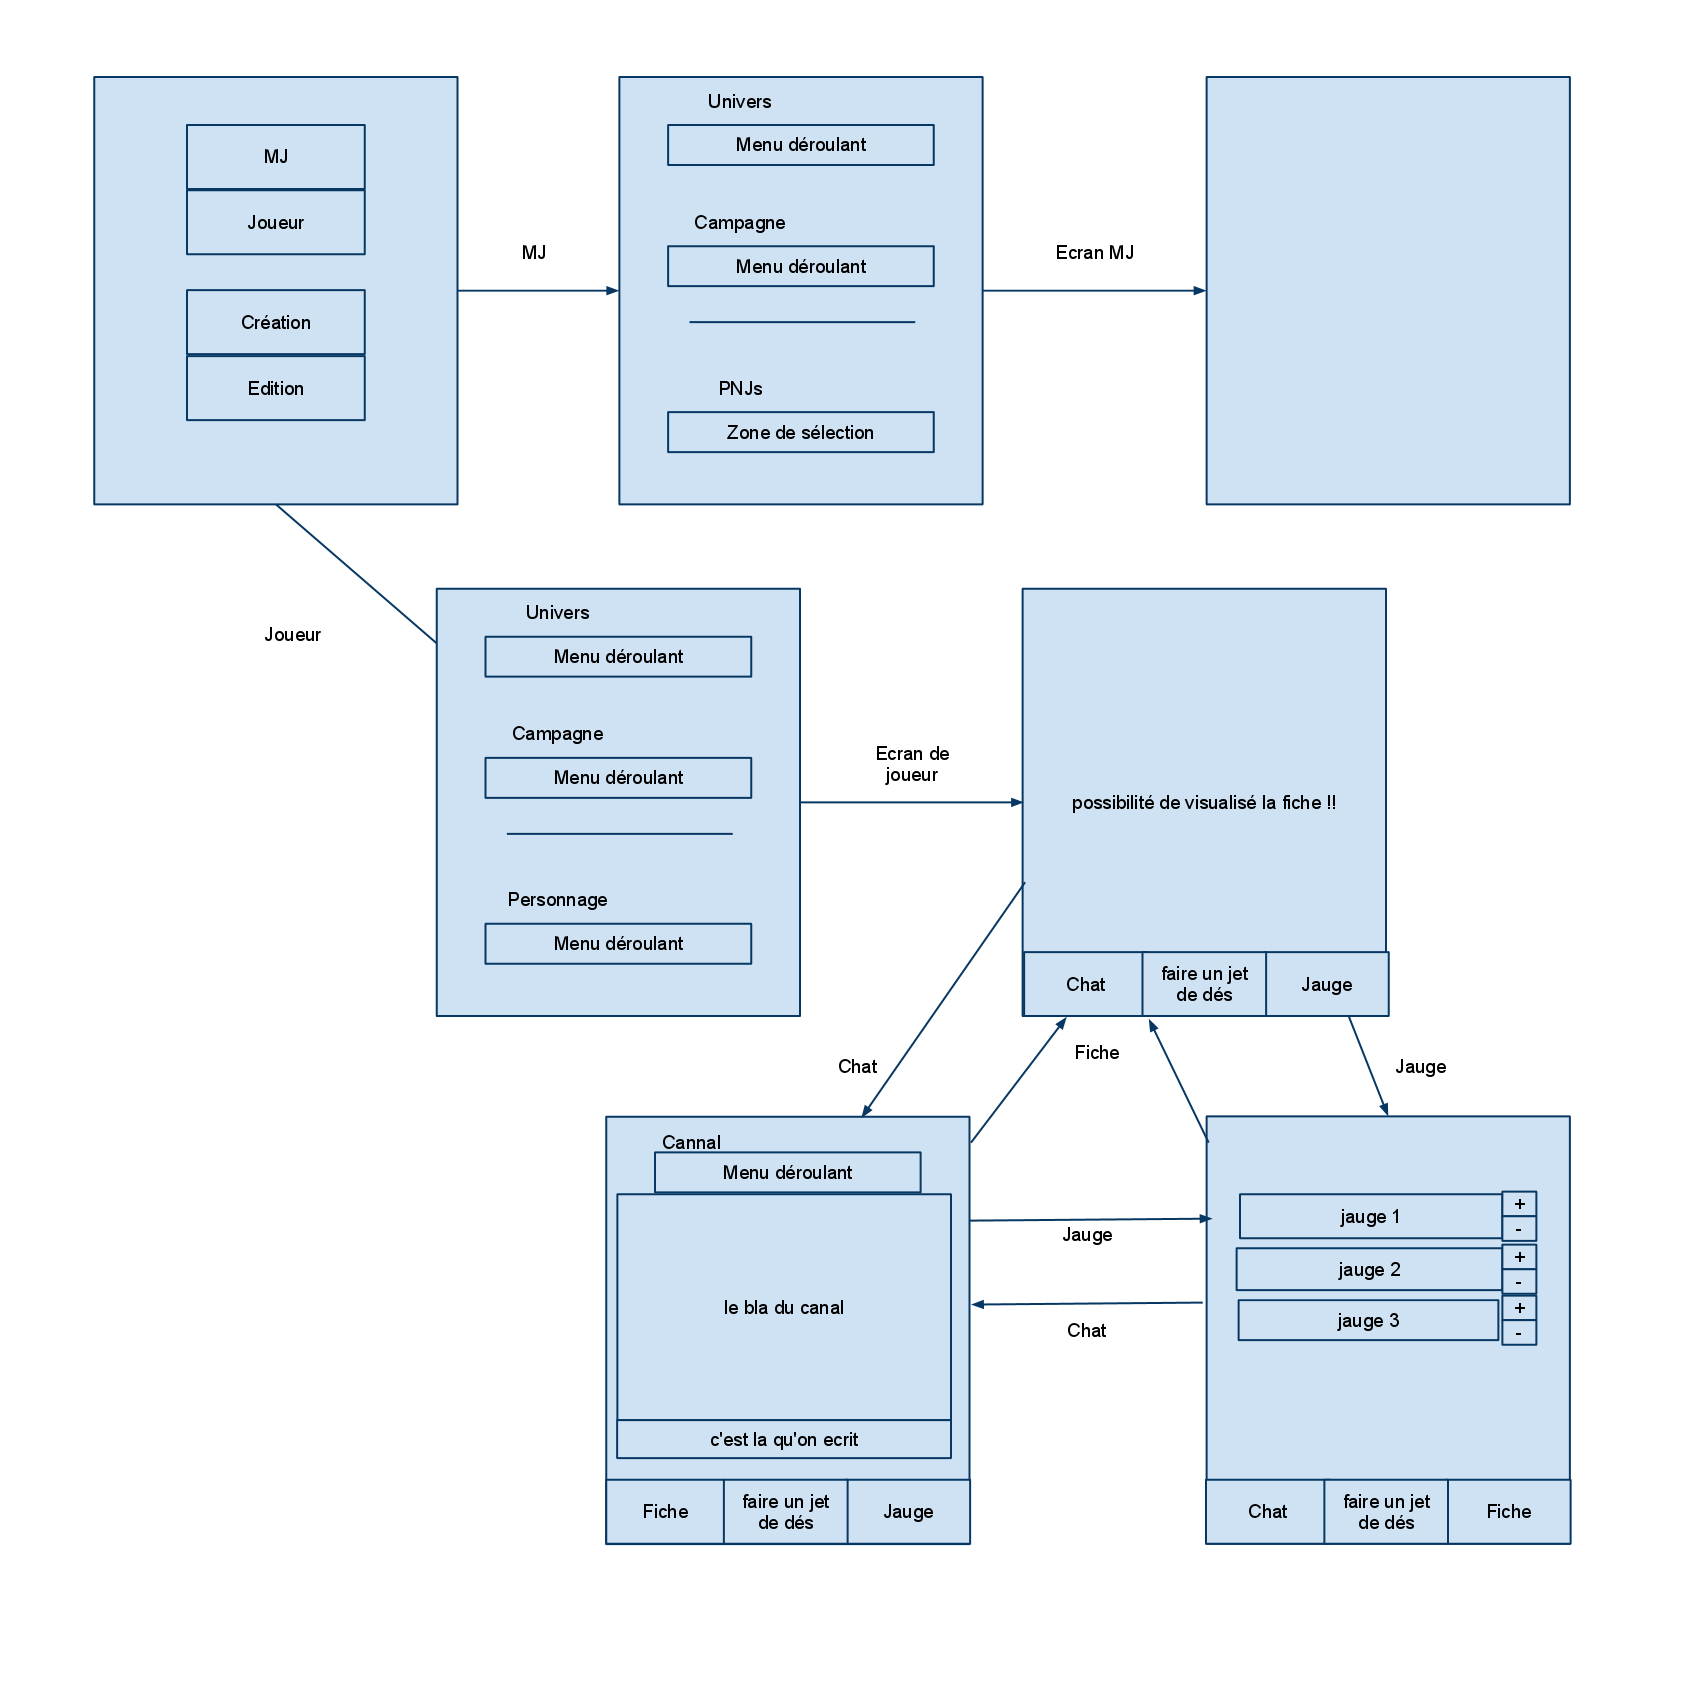
\includegraphics[height=14cm,width=15cm]{image/screen2.png}
  		\caption{Enchainement logique des écrans}
  		\label{screen2}
\end{figure}

La capture \ref{screen2} permet de voir plus en détail la logique d'enchainement des écrans, 
avec l'affichage des fonctionnalités clés, et le fait que l'on puisse rapidement basculé rapidement d'un écran à un autre.
On le voit aussi la présence d'une partie jauge, les éléments d'une fiche qui évoluent à chaque instant du jeu, 
élément pas toujours regroupé dans une fiche, qui là pour le coup se "trouvent" facilement. 

\begin{figure}[h]
  	
  		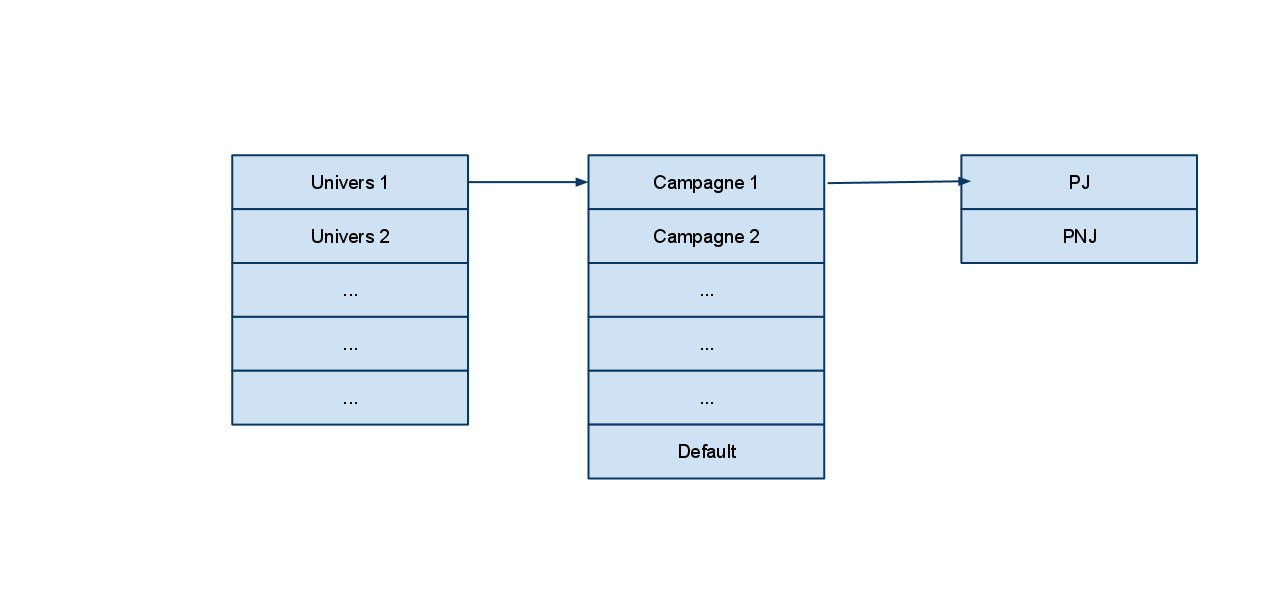
\includegraphics[height=14cm,width=15cm]{image/screen3.png}
  		\caption{Gestion des fiches}
  		\label{screen3}
\end{figure}

La capture \ref{screen3} montre la gestion des fiches de personnage en fonction de l'univers (jeu en général), de 
la campagne, nom donné à un ensemble de scénario généralement cohérent dans lesquels évolue des personnages, une histoire. 
Ensuite une gestion joueur et non joueur pour un meilleur tri des informations, et affiner les critère de sélections.

\begin{figure}[h]
  	
  		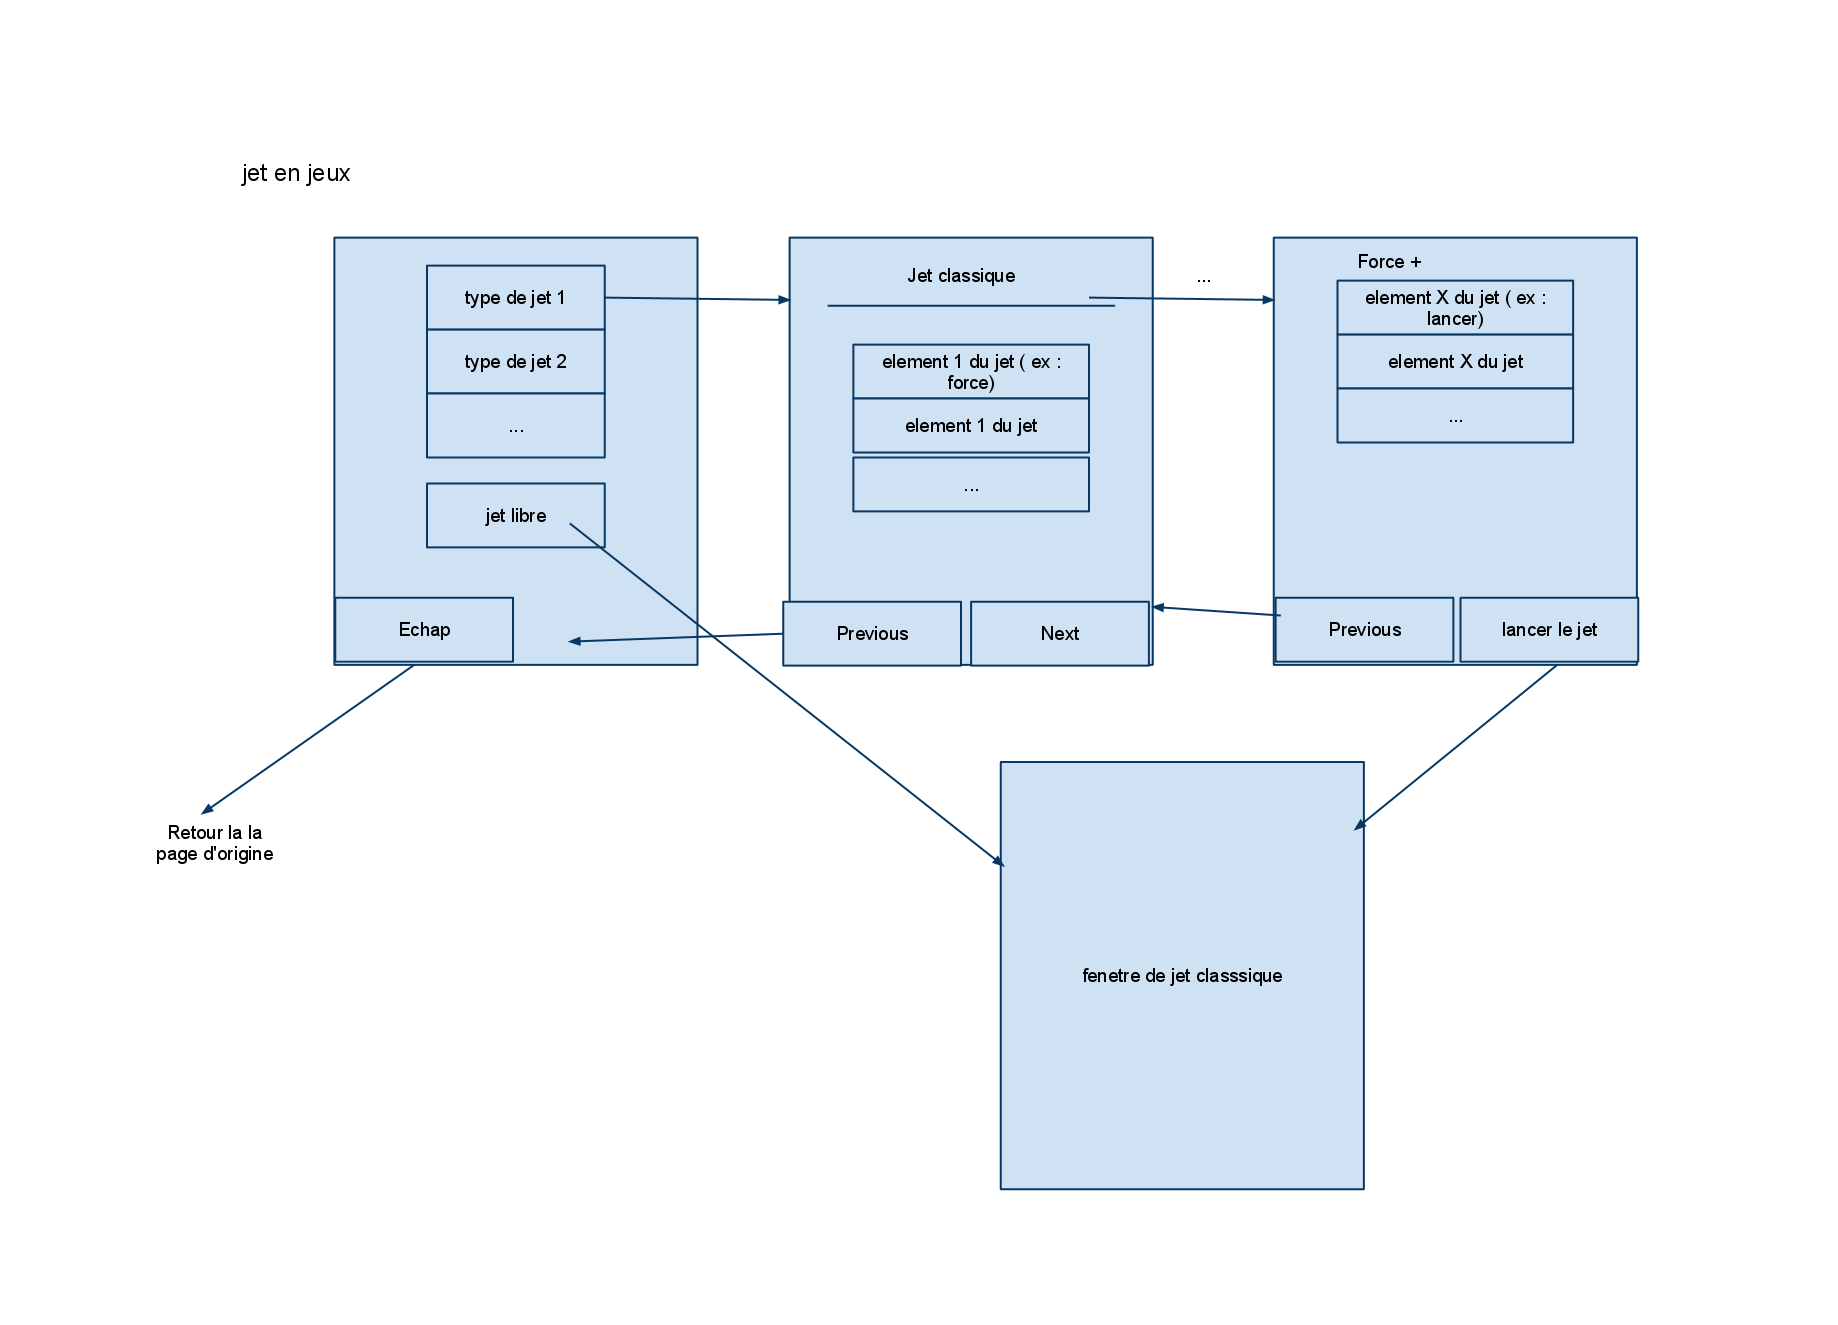
\includegraphics[height=14cm,width=15cm]{image/screen4.png}
  		\caption{Gestion des jets en jeu}
  		\label{screen4}
\end{figure}

La capture \ref{screen4} montre le choix du type du jet de dés, qui nous permet de gérer en partie
les rêgles d'un jeu, et donc d'avoir des jets cohérents. Ensuite celui qui veut faire le jet
choisis ses élements du jet.

\begin{figure}[h]
  	
  		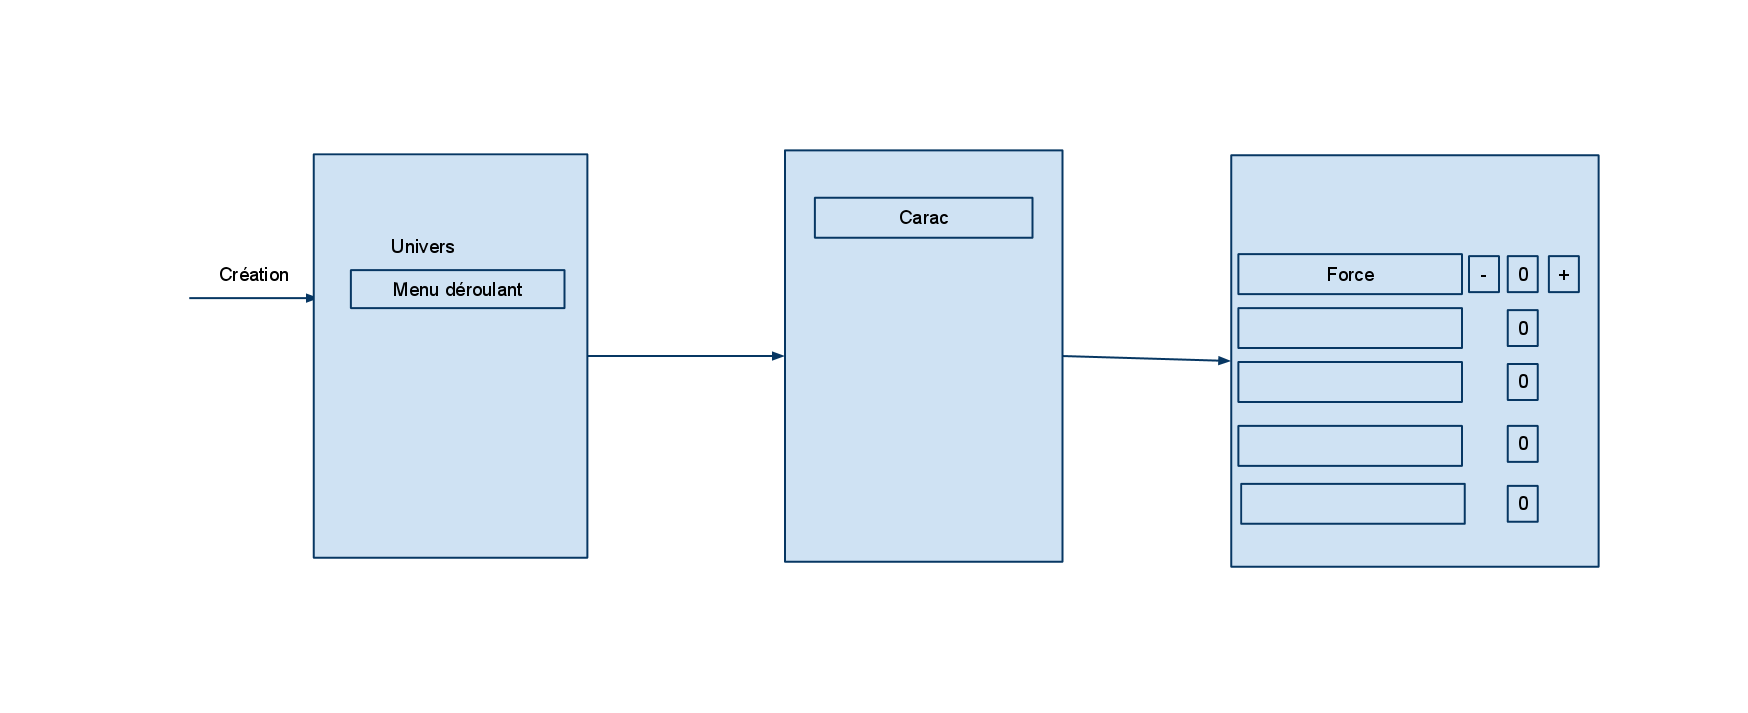
\includegraphics[height=14cm,width=15cm]{image/screen5.png}
  		\caption{Création de personnage}
  		\label{screen5}
\end{figure}

La capture \ref{screen5} nous montre la création de personnsage avec l'affichage, des différents 
éléments de fiche à modifier à la création, l'écran ne suppose aucune gestion de rêgle de création 
de personnage, et c'est le cas, l'application ne supporte pas le rêgle de création.


\section{Lucid 4}

\subsection{Définition}

Cette étape de la méthode est une étape presque introspective, elle permet de
revenir, sur les étapes précédentes par rapport au retour client sur le
prototypage. Et par la même de pouvoir commencer à établir le plan de
construction de l'application au niveau des fonctionnalités. Il s'agit de
plannifier les taches de dévellopement. 

\subsubsection{Notre organisation}

Pour cette étape de la méthode nous avons tous remis en parrallèle, les concepts initiaux 
du produit, les réactions et analyse des utilisateurs et les exquisses. Nous avons pu faire remonter des
remarques sur les première exquisses, ainsi que nous rendre compte de ce qui était possible concrétement
avec la plateforme android.

Cette étape à permis d'affiner clairement les fonctionnalités et de commencer à appréhender la façon dont elles 
allaient éxister concrétement sous une plateforme mobile comme android. Remettre à plat tout celà
nous a permis de dégager les grosses de dévellopements que nous avions à faire.

Les travaux de définition et de modélisation des éléments liés au jeu de rôle comme les éléments commun à toutes les fiches,
la conception de modèle suffisament large pour assurer la prise en charge du plus de jeu possible, cette tâche à été commune à tous
les membres de l'équipe. Nous y avons tous participé puisque nous avions tous des expériences différentes et qu'elles étaient relativement complémentaire.

Nous avons défini aussi l'architecture globale de l'application, architecture de type composant, avec des composants comme:
\begin{itemize}
  \item Composant Dé
  \item Composant gestion des fiches en xml
  \item Composant connectivité(support bluetooh/wifi)
\end{itemize}

Ces composants sencé être élémentaire devant permettre la construction de l'application par dessus, avec l'application du pattern 
adapter, pour permettre un éventuel réutilisation de ces composants, et surtout une relecture de code plus aisée.

C'est pendant cette étape que nous avons choisis de ne pas implémenter la partie connectivité de l'application,
la méconnaissance du support android nous ralentissant déja pour les fonctionnalités plus simple.

Durant cette étape nous avons tous travailler à enrichir nos connaissances sur android, en mettant en place 
des mini tutos et en recoupant les informations que nous avons receuilli sur la plateforme.

De plus pour travailler en colaboration nous avons choisi de mettre en place un gestionnaire de version sous google code qui nous
as accompagné tout du long du devellopement. De plus nous avions des réunions régulière sur Skype pour coordonnéer nos efforts 
de devellomepent. Et nous avions en paralèlle googledocs pour certain document comme les esquisses.

\section{Lucid 5}

\subsection{Définition}

Cette étape de la méthode est l'implémentation de l'application. C'est donc dans
cette étape que l'interface est écrite en parrallèle avec le code effectif des
fonctions. C'est aussi le moment où l'on commence à écrire les documentations et
quelques structures communautaire autour de l'outil. C'est vraiment à ce moment
là que l'on rentre dans un cycle logiciel avec du concret informatiquement
parlant.

\subsection{L'implémentation}

Pour l'implémentation, il y a plusieurs phases, d'abord la définition et l'écriture des composants
en java sur lesquels l'application devaient s'appuyer. Ce fut la première étape de devellopement.
Cette première étape n'a pas forcément posé de problème au cours du projet.

Ensuite le dévellopement s'est continué en s'appuyant sur ces premiers module de base.


\subsubsection{Modules de base}

Ces modules sont utilisés par l'interface graphique. Ils fournissent des
fonctionnalités propres au coeur de l'application.

\begin{itemize}
  \item DiceModule : il fournit différents méthodes permettant d'effectuer
  plusieurs types de jet de dés.
  \item FicheModule : il permet d'enregistrer/charger une fiche de personnage, à
  partir d'un modèle de fiche, ou bien à partir d'une fiche même. Cela comprend
  aussi le parseur xml nécessaire à ces opérations.
  \item SystemModule : idem que FicheModule, mais pour un système de règle.
\end{itemize}

\subsubsection{IHM Android}

Pour expliciter notre interface androïd, nous avons fait le choix d'expliquer
les types d'écran utilisés et non chacun d'eux afin d'être plus synthétique.

\paragraph{Interface à boutons}
~\\
~\\
 Ce type d'interface est utilisé dans la page d'accueil de notre application.
 Il permet un choix simplifié pour l'utilisateur.

\paragraph{Interface avec listeView}
~\\
~\\
Nous avons utilisé les listView dans des écran de séléction. Celui-ci est rempli
dynamiquement avec du texte provenant du parsing de fiche ou d'un système de
règles. Chaque élément est cliquable afin d'avancer dans le processus
d'application. Par exemple, la sélection d'un des éléments d'un jet de dé.\\

De plus, nous avons utilisé cet outil graphique afin de modifier des valeurs
associées par exemple à des compétences. Nous avons donc personnalisé chaque
ligne de la listView à l'aide d'un Adapter. Cette ListView ne comprend donc plus
uniquement du texte mais des boutons ou encore des EditText.

\paragraph{Interface avec Spinner}
~\\
~\\
L'utilisation des Spinner a été nécessaire pour faciliter les choix de
l'utilisateur. Ces Spinners permettent une séléction filtrées des univers et des
campagnes. Par exemple, lorsque l'utilisateur veut voir une fiche, il
sélectionne dans un premier temps l'univers. Puis, il sélectionnera les
différentes campagnes disponible par rapport à cet univers et enfin les fiches
disponibles pour cet univers et cette campagne.

\paragraph{Interface du jet de dé}
~\\
~\\
Ce type d'interface permet d'effectuer un jet de dé utilisant différents outils
graphiques androïd. Soit en le parametrant totalement, soit après avoir
sélectionné les différents éléments du jet.

\section{Lucid 6}

\subsection{Définition}

Cette étape de la méthode est l'évaluation externe du projet. Elle s'accompagne
généralement de la diffusion d'une première version public du produit qui
normalement est proche de la version finale tant par l'aspect que par ses
fonctionnalités.
Cette étape permet de lever les dernières remarques du public visé, et de
corriger les bugs induit par la différence d'utilisation des utilisateurs finaux
par rapport à l'utilisation des devellopeurs.


\subsection{Plan d'évalution}

Pour l'évalutation de notre application nous avons pensé à plusieurs niveau d'écoute
des utilisateurs. Nous proposons une application qui se veut pour un large panel 
de joueurs et de MJ avec des attentes différentes.

Nous avons pensé à trois niveau d'évaluation par les utilisateurs, trois type de niveau de communication
 avec la communauté. Un pour les MJ, utilisateur amené à faire évoluer les modèles de fiche modèle de système
et les contraintes d'affichage pour information multiple.

Un autre pour les "simples" utilisateur, client/consommateur voulant s'en servir pour se séparer
du support physique pour plus de facilité. La synchro de fiche, édition, jeu, jet de dés etc.
Et donc pour ce "niveau" l'écoute de joueur avancé ayant dépassé la phase d'apprentissage 
du média, pour une ergonomie optimal pour l'utilisation de l'application. 

Ensuite le dernier type correspondrait aux retour des utilisateurs ne maîtrisant que peu le support
android. Donc presque la cible privilégié de cette approche sur le retour, le but étant d'être particulièrement
à l'écioute de ces utilisateurs, afin qu'ils prennent bien en main l'application, mettre en place un apprentissage
efficace pour faire d'eux des utilisateurs "simple" 

Le but final est un nivellement du niveau des utilisateurs vers le niveau simple, ou tout du moins 
qu'a terme il n'y ait que deux niveaux d'utilisateur, que très vite tout utilisateur novice devienne rapidement
un utilisateur simple pour qu'il puisse profiter pleinement de l'application, que celà ne le ralentisse pas lors 
des parties, que ce ne soit pas un handicap.

Un des avantages à être sur une plateforme tactile c'est que l'aprentissage est assez rapide et simple
pour peu que l'application ait bien été construite, ce que nous espérons dans notre cas.


\section{Conclusion}

Lucid est une méthode résolument ethno centré, c'est un fait indéniable, nous l'avons constaté
du fait de la proximité nécessaire avec les futurs utilisateur. C'est un avantage certain pour 
l'acceptation finale du produit par l'utilisateur. 

Le soucis serait que cette méthode par certain aspect, entre en conflit avec les méthodes
d'ingénièrie logiciel classic, bien qu'il y ait des similitudes, il y a quelques incompatiblités.

On gagne pourtant à l'utiliser, on a  plus de chance que le produit soit accepté et
conforme à ce que l'utilisateur final va vouloir, mais le temps nécessaire plus
long que un cycle "classique'' implique potentiellement plus d'argent à investir
pour le client, et généralement ça ne leur plait pa ça. L'idéal serait une méthode de devellopement 
intégrant l'ethno centrisme de lucid avec la performance de d'autres méthodes.

Un autre soucis que l'on peut remarquer avec lucid c'est l'aspect communication avec le client,
allant de pair avec l'analyse ses besoins et la transcription en élément informatique concret et utilisable.
Cet aspect social, la communication des dévellopeurs avec les client généralement compliqué, ici la méthode 
est basé sur cet aspect. Or en fait actuellement il ne faut pas se leurer, le marché des informaticiens
est saturé par des gens associaux qui ont naturellement des problèmes de communication.

Conclusion cette méthode est très intéressante, mais peut être trop utopiste compte tenu 
de la situation actuelle.

  
  
\end{document}
